% One look for every architecture figure. Change a colour or font here, once.
\PassOptionsToPackage{table}{xcolor}
\usepackage[T1]{fontenc}
\usepackage{lmodern}
\renewcommand{\familydefault}{\sfdefault}
\usepackage{amsmath}
\usepackage{array}
\usepackage{graphicx}
\usepackage{fontawesome5}
\usepackage{tikz}
\usetikzlibrary{positioning, arrows.meta, fit, backgrounds, calc,
  decorations.pathreplacing}

% colour says where the weights came from, nothing else
\definecolor{preEdge}{RGB}{0,94,150}      % pretrained weights
\definecolor{preFill}{RGB}{214,232,245}
\definecolor{newEdge}{RGB}{176,92,0}      % new weights, trained from scratch
\definecolor{newFill}{RGB}{253,229,196}
\definecolor{opEdge}{RGB}{120,120,120}    % no weights
\definecolor{opFill}{RGB}{236,236,236}
\definecolor{ink}{RGB}{35,35,35}
\definecolor{note}{RGB}{90,90,90}
\definecolor{groupFill}{RGB}{245,245,245}
\definecolor{stripe}{RGB}{243,243,243}
% boxes drawn on photos: Okabe-Ito, readable on grass
\definecolor{strikerBox}{RGB}{0,114,178}
\definecolor{batBox}{RGB}{204,121,167}
\definecolor{cropBox}{RGB}{230,159,0}

% the icon says whether the weights move during training
\newcommand{\frozen}{{\color{ink}\faSnowflake[regular]}}
\newcommand{\trained}{{\color{ink}\faFire}}

% a small filled square for legends; no tikz inside tikz
\newcommand{\swatch}[2]{{\setlength{\fboxsep}{0pt}\setlength{\fboxrule}{0.6pt}%
  \fcolorbox{#1}{#2}{\rule{0pt}{1.4ex}\rule{2.2ex}{0pt}}}}
\newcommand{\archlegend}{\swatch{preEdge}{preFill}~pretrained weights\quad
  \swatch{newEdge}{newFill}~new weights\quad
  \swatch{opEdge}{white}~no weights\qquad
  \frozen~frozen\quad \trained~trained}

% tensor sizes
\newcommand{\by}{\ensuremath{\times}}
\newcommand{\sq}{\textsuperscript{2}}
\newcommand{\dims}[1]{#1}
\newcommand{\arrowto}{\ensuremath{\to}}

\tikzset{
  every node/.style={font=\footnotesize, text=ink},
  flow/.style={-{Stealth[length=2.2mm, width=1.7mm]}, line width=0.75pt,
    draw=ink},
  box/.style={rounded corners=2pt, line width=0.7pt, align=center,
    minimum height=8mm, inner sep=3pt,
    execute at begin node={\hyphenpenalty=10000\exhyphenpenalty=10000}},
  pre/.style={box, draw=preEdge, fill=preFill},
  new/.style={box, draw=newEdge, fill=newFill},
  op/.style={box, draw=opEdge, fill=white},
  group/.style={rounded corners=3pt, draw=opEdge, dashed, line width=0.5pt,
    fill=groupFill, inner sep=4pt},
  grouplabel/.style={font=\scriptsize, text=note, inner sep=1pt},
  % a tensor size, sitting on its arrow so it never crosses a line
  dim/.style={font=\scriptsize, text=ink, fill=white, draw=opEdge!55,
    line width=0.3pt, rounded corners=1.5pt, inner sep=1.1pt},
  size/.style={font=\scriptsize, text=note, inner sep=1.5pt,
    execute at begin node={\hyphenpenalty=10000\exhyphenpenalty=10000}},
  tag/.style={font=\scriptsize\bfseries, inner sep=1pt},
  legend/.style={font=\scriptsize, text=note, inner sep=2pt},
  frame/.style={inner sep=0pt, draw=ink!55, line width=0.3pt},
  letter/.style={font=\footnotesize\bfseries, inner sep=0pt},
  % a box opening up into the table that lists its options
  cone/.style={fill=#1, fill opacity=0.45, draw=none},
  conelink/.style={draw=opEdge!80, line width=0.4pt, densely dashed},
  bone/.style={line width=1.0pt, draw=white, line cap=round},
  guess/.style={line width=0.8pt, draw=white, dash pattern=on 1.6pt off 1.2pt},
  joint/.style={fill=cropBox},
  guessjoint/.style={fill=white},
}

% a clip as a deck of three of its frames; #1 name, #2 where, #3 width
\newcommand{\clipdeck}[3]{%
  \node[frame] (#1-c) at ($(#2)+(0.22,0.22)$)
    {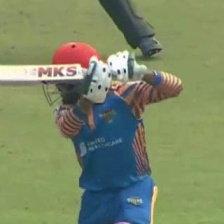
\includegraphics[width=#3]{img/crop15.jpg}};
  \node[frame] (#1-b) at ($(#2)+(0.11,0.11)$)
    {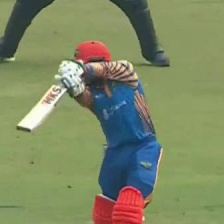
\includegraphics[width=#3]{img/crop08.jpg}};
  \node[frame] (#1-a) at (#2) {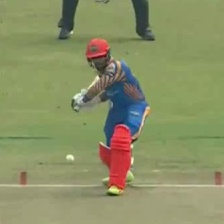
\includegraphics[width=#3]{img/crop01.jpg}};
  \node[fit=(#1-a)(#1-b)(#1-c), inner sep=0pt] (#1) {};
}

% a table card: a header band in the colour of the box it opens up.
% #1 name, #2 top-left corner, #3 band fill, #4 edge, #5 title, #6 a tabular
\newcommand{\card}[6]{%
  \node[anchor=north west, inner sep=0pt, fill=white, font=\scriptsize]
    (#1) at ([yshift=-5mm]#2) {#6};
  \node[fit={(#1.north west)([yshift=5mm]#1.north east)}, inner sep=0pt,
    fill=#3] (#1-head) {};
  \node[anchor=west, inner sep=0pt, font=\footnotesize\bfseries]
    at ([xshift=4pt]#1-head.west) {#5};
  \draw[#4, line width=0.7pt] (#1-head.north west) rectangle (#1.south east);
  \draw[#4, line width=0.5pt] (#1-head.south west) -- (#1-head.south east);
}
% rows inside a card
\newcommand{\cardrule}{\arrayrulecolor{opEdge!60}\hline}
\newcommand{\grouprow}[2]{\rowcolor{white}%
  \multicolumn{#1}{l}{\rule{0pt}{2.6ex}\textbf{\color{note}#2}}\\}
\newcolumntype{P}[1]{>{\raggedright\arraybackslash}p{#1}}
\newcommand{\cardtable}[2]{{\setlength{\tabcolsep}{4pt}%
  \hyphenpenalty=10000\exhyphenpenalty=10000%
  \renewcommand{\arraystretch}{1.12}\rowcolors{2}{white}{stripe}%
  \begin{tabular}{#1}#2\end{tabular}}}
% the shaded zoom from a box (#1) down to its card (#2), colour #3
\newcommand{\zoomto}[3]{%
  \begin{scope}[on background layer]
    \fill[cone=#3] (#1.south west) -- (#1.south east) --
      (#2-head.north east) -- (#2-head.north west) -- cycle;
  \end{scope}
  \draw[conelink] (#1.south west) -- (#2-head.north west);
  \draw[conelink] (#1.south east) -- (#2-head.north east);
}
